\documentclass[a4paper,12pt]{article} % тип документа

% report, book

% Рисунки
\usepackage{graphicx}
\usepackage{wrapfig}

\usepackage{hyperref}
\usepackage[rgb]{xcolor}
\hypersetup{				% Гиперссылки
    colorlinks=true,       	% false: ссылки в рамках
	urlcolor=blue          % на URL
}

%  Русский язык

\usepackage[T2A]{fontenc}			% кодировка
\usepackage[utf8]{inputenc}			% кодировка исходного текста
\usepackage[english,russian]{babel}	% локализация и переносы


% Математика
\usepackage{amsmath,amsfonts,amssymb,amsthm,mathtools} 


\usepackage{wasysym}

\author{Анна Назарчук Б02-109}
\title{1.2.5 Исследование вынужденной регулярной прецессии гироскопа}
\date{}
\begin{document}
\maketitle
\section{Теоретические сведения}
Уравнение движения твердого тела:
\begin{equation}
\frac{\overrightarrow{dp}}{dt}=\overrightarrow{F}
\end{equation}
\begin{equation}
\frac{\overrightarrow{dL}}{dt}=\overrightarrow{M}
\end{equation}
Так как сила $\overrightarrow{F}$ не зависит от угловой скорости, а момент сил $\overrightarrow{M}$ - от скорости поступательного движения, то уравнения движения можно рассматривать отдельно.
\begin{equation}
\overrightarrow{L}=\overrightarrow{i}I_x\omega_x+\overrightarrow{j}I_y\omega_y+\overrightarrow{k}I_z\omega_z
\end{equation}
Гироскоп  - быстро вращающееся тело, для которого, например:
\begin{equation}
I_z\omega_z\gg I_x\omega_x, I_y\omega_y
\end{equation}
Уравношенный гироскоп - тот, у которого центр масс неподвижен.
Если момент внешних сил действует в течение короткого промежутка времени, то:
\begin{equation}
|\Delta \overrightarrow{L}|=|\int \overrightarrow{M}dt|\ll |\overrightarrow{L}|
\end{equation}
Рассмотрим маховик, вращающийся вокргу оси $z$ (рис. \ref{маховик}). Будем считать, что:
\begin{equation}
\omega_x=\omega_0,\quad		\omega_y=0, \quad	\omega_z=0
\end{equation}
\begin{figure}[h!]
\begin{center}
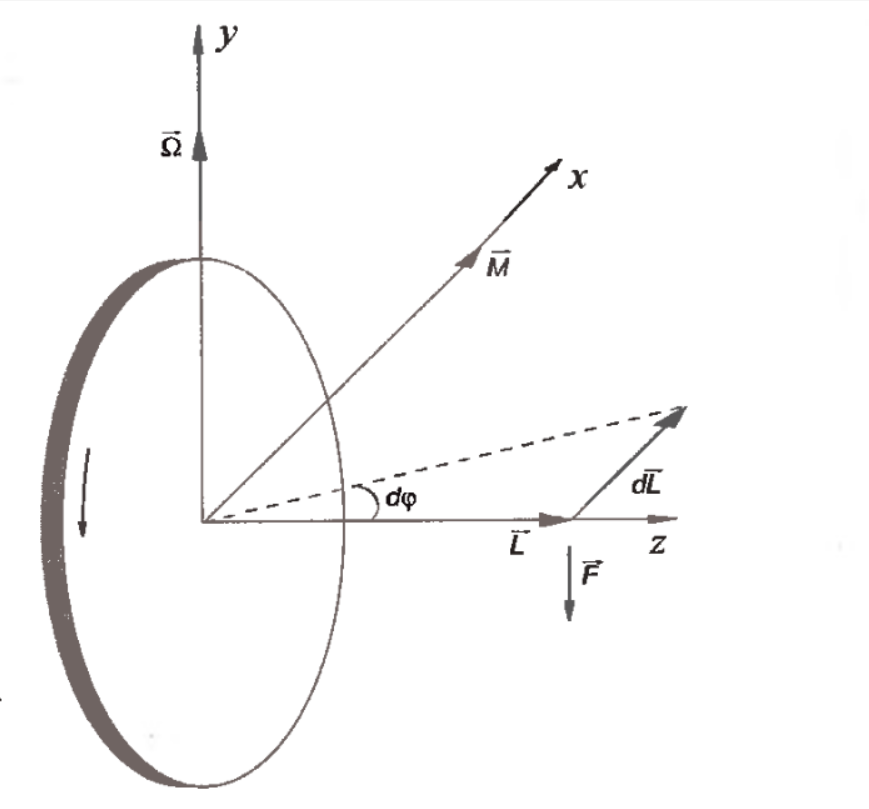
\includegraphics[width=0.5\textwidth]{Маховик}
\end{center}
\caption{Маховик} \label{маховик}
\end{figure}
Пусть ось вращения повернулась на угол $d\varphi$ в плоскости $zx$:
\[d\varphi=\Omega dt\]
Будем считать, что $L_\Omega \ll \L_{\omega_0}$ 
Это означает, что момент импульса маховика изменится только по направлению:
\begin{equation}
|\overrightarrow{dL}|=Ld\varphi=L\Omega dt
\end{equation} 
Изменение направлено вдоль оси x, поэтому $\overrightarrow{dL}$ можно представить:
\begin{equation}
\frac{\overrightarrow{dL}}{dt}=\overrightarrow{\Omega}\times\overrightarrow{L}
\end{equation}
С учетом уравнения вращательного движения:
\begin{equation}
\overrightarrow{M}=\overrightarrow{\Omega}\times\overrightarrow{L}
\end{equation}
Под действием момента $\overrightarrow{M}$ ось гироскопа медленно вращается вокруг оси $y$ с угловой скоростью $\Omega$ - регулярная прецессия гироскопа.
Скорость в случае движения уравновешенного гироскопа под действием моментов сил подвешенных грузов:
\begin{equation}
\label{связь омег}
\Omega = \frac{mgl}{I_z\omega_0},
\end{equation}
где $l$ - расстояние от центра карданова подвеса до точки крепления груза на оси гироскопа (рис. \ref{схема})
\begin{figure}[h!]
\begin{center}
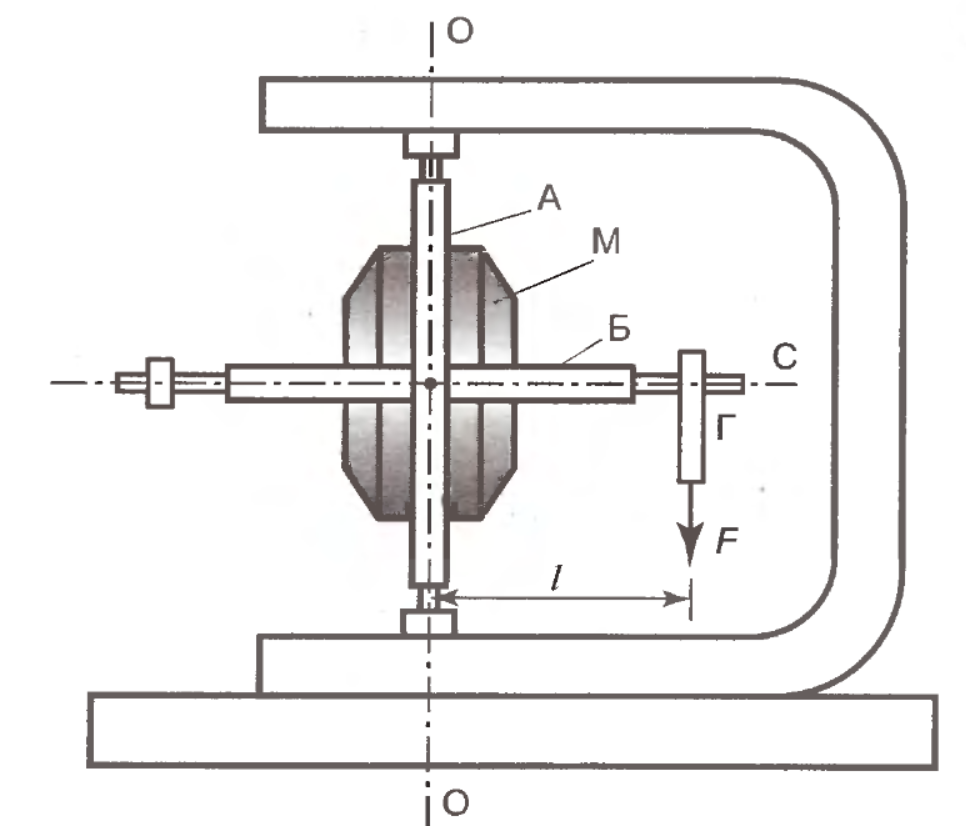
\includegraphics[width=0.5\textwidth]{Схема}
\end{center}
\caption{Схема экспериментальной установки} \label{схема}
\end{figure}


Силы трения не лежат в плоскости осей вращения, поэтому они могут изменять момент импульса и по направлению, и по величине. Для ротора действие сил трения скомпенсировано действием электромотора. В результате действия нескомпенсированных сил трения в осях карданова подвеса ось гироскопа будет опускаться в направлении груза.

Момент инерции ротора относительно оси симметрии $I_0$ измеряется по крутильным колебаниям на жесткой проволоке. 
\begin{equation}
T_0 = 2\pi\sqrt{\frac{I_0}{f}},
\end{equation}
где $f$ - модуль кручения проволоки
Чтобы исключить $f$ можно подвесить цилиндр с известными размерами и массой:
\begin{equation}
I_0=I_\text{ц}\frac{T_0^2}{T_\text{ц}^2}
\end{equation}

\section{Измерения и обработка данных}
\subsection{Исследование зависимости скорости прецессии от момента сил}
Отклонив рычаг на 5-6 градусов вверх и подвесив к нему груз, найдем скорость регулярной прецессии и скорость опускания рычага. Результаты измерения с постоянным моментом сил (для измерения погрешности измерений) и разными представлеными в таблице \ref{момент} 

\begin{table} \label{момент} \caption{Измерения с разными моментами сил} \begin{tabular}{|c|c|c|c|c|} \hline m, г & N оборотов & T, с & $\Omega$, 1/с & $\Delta\alpha$, 1/c \\ \hline 57 & 2 & 364 & 0.035 & 0.306 \\ \hline 92 & 2 & 220 & 0.057 & 0.168 \\ \hline 92 & 2 & 223 & 0.057 & 0.113 \\ \hline 92 & 2 & 221 & 0.057 & 0.118 \\ \hline 92 & 2 & 217 & 0.058 & 0.173 \\ \hline 92 & 2 & 221 & 0.057 & 0.135 \\ \hline 116 & 3 & 261 & 0.072 & 0.206 \\ \hline 142 & 3 & 215 & 0.088 & 0.19 \\ \hline 180 & 4 & 224 & 0.112 & 0.201 \\ \hline 219 & 5 & 232 & 0.135 & 0.19 \\ \hline 273 & 6 & 223 & 0.169 & 0.157 \\ \hline 341 & 8 & 236 & 0.213 & 0.206 \\ \hline 74 & 2 & 271 & 0.046 & 0.124 \\ \hline \end{tabular} \end{table}

Из результатов таблицы \ref{момент} можно найти систематическую составлющую погрешности $\Omega$, связанную с неточностью определения времени:
\begin{equation}
\frac{\sigma_\Omega}{\Omega}= 0.027
\end{equation}

Исходя из полученной случайной погрешности и результатов в таблице (\ref{момент}) построим график зависимости $\Omega$ от $M$ (рис. \ref{график})
\begin{figure}[h!]
\begin{center}
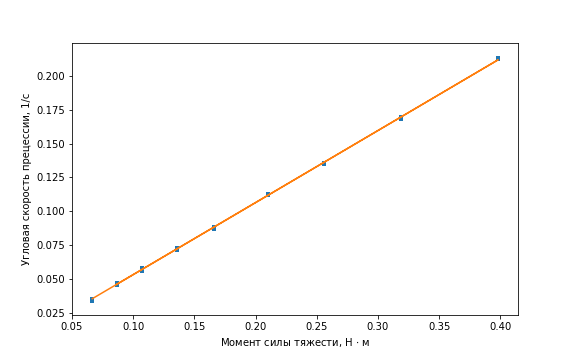
\includegraphics[width=\textwidth]{График}
\end{center}
\caption{Зависимость $\Omega$ от $M$} \label{график}
\end{figure}

\subsection{Измерение момента инерии ротора}

Характерные размеры цидиндра: $m = 1617.8 \text{ г}, d = 78.1 \text{ мм} $ 

Из данных можно сказать, что $I_ \text{ц} = 0.00123349
 \text{ кг} \cdot \text{м}^2$
Результаты измерений периода крутильных колебаний с ротором и цилиндром представлены в таблице \ref{инерция}

\begin{table} \caption{Измерения момента инерции ротора}
\label{инерция} \begin{tabular}{|c|c|c|c|} \hline N оборотов цилиндра & N обор. ротора & T вращения ротора, с & T вращ. цилиндра,c \\ \hline 11 & 10 & 3 & 3.955 \\ \hline 10 & 10 & 3 & 4 \\ \hline 10 & 10 & 3.26 & 4 \\ \hline 10 & 10 & 3 & 4 \\ \hline 10 & 10 & 3 & 4 \\ \hline \end{tabular} \end{table}
Из приведенных измерений можно сказать, что:
\begin{equation}
I_0 = (0.78 \pm   0.03)\cdot 10^{-3} \text{кг} \cdot \text{м}^2
\end{equation}

\subsection{Рассчет частоты вращения и момента сил трения}
По формуле \ref{связь омег} можно понять, что $\nu_0$ (частота вращения)- величина, обратно пропорциональная наклону графика на рис. \ref{график}.
С помощью МНК найдем наклон графика $a$, а из него $\nu_0$:
\[\nu_0 = \frac{1}{2\pi\cdot aI_0} =385.71   \pm  12.73\text{ }c^{-1}\]

Определим момент сил трения. Для каждого эксперимента будем измерять высоту опускания груза, тем самым измерив угол опускания за период измерения.
\begin{equation}
M_\text{тр} = \frac{mgl\Delta\alpha}{2\pi N},
\end{equation}
где $\Delta\alpha$ - угол опускания за N оборотов регулярной прецессии.
Данные об измерения в таблице \ref{момент}. Погрешность измерения $\Delta\alpha$ определим исходя из полученных значений при неизменной массе груза, а следовательно и момента силы тяжести. В связи с неточным определением смещения по высоте и времени, погрешность момента силы трения сравнительно остальных измерений высока:
\begin{equation}
M_\text{тр} = 1.37 \pm 0.26 \text{ мН} \cdot \text{ м}
\end{equation}

\subsection{Определение частоты вращения ротора по фигурам Лиссажу}
Если на один вход осциллографа подать ЭДС во второй обмотке статора гироскопа, а на второй - напряжение с генератора, то при совпадении частот можно увидеть эллипс.
Для достижения более неподвижного эллипса, можно на короткое время выключить питание гироскопа, чтобы ток первой обмотки не мешал измерениям. Таким образом:
\begin{equation}
\nu = 395 \text{ Гц}
\end{equation}
Данное значение частоты лежит в пределах погрешности частоты, измеренной с помощью эксперимента с вращением гироскопа.

Проверим справедливость соотношения: $L_\Omega \ll \L_{\omega_0}$. Значения моментов инерции ротора по разным осям не отличаются по порядку, а угловые скорости:
\[\Omega \approx 0.06 \text{ } 1/c \ll \omega_0 \approx 2400 \text{  }1/c\]
поэтому предположенное соотношение верно.

\section{Вывод}
Установлена зависимость скорости вынужденной прецессии от величины момента сил, действующих на ось гироскопа; определена скорость вращения ротора гироскопа и сравнить ее со скоростью, рассчитанной по скорости прецесии.
\end{document}